\chapter{Test del software}
\begin{redbar}
Il \textbf{testing} ha l’obiettivo di mostrare che un programma svolge il compito per cui è stato progettato e di identificare eventuali difetti prima che venga messo in uso. Quando si testa il software, si esegue un programma utilizzando dati artificiali. Si verificano i risultati del test per individuare errori, anomalie o informazioni sulle caratteristiche non funzionali del programma. 
\end{redbar}
Testare il software implica due obiettivi principali:
\begin{enumerate}
    \item Dimostrare al team di sviluppo e al cliente che il software soddisfa i requisiti. Per il software personalizzato, ciò significa che dovrebbe esserci almeno un test per ogni requisito nel documento dei requisiti. Per i prodotti software generici, ci dovrebbero essere test per tutte le funzionalità del sistema che verranno incluse nella versione finale.
    \item Trovare input o sequenze di input in cui il comportamento del software è scorretto, indesiderato o non conforme alle specifiche. Questi problemi sono causati da difetti (bug) nel software. Quando si testano i software per trovare difetti, si cerca di eliminare comportamenti indesiderati come crash di sistema, interazioni indesiderate con altri sistemi, calcoli errati e corruzione dei dati.
\end{enumerate}
La prima attività è il testing di validazione, dove ci si aspetta che il sistema funzioni correttamente usando casi di test che riflettano l’uso previsto del sistema. La seconda è il testing per la rilevazione dei difetti, dove i casi di test sono progettati per esporre i difetti. Non c'è una separazione netta tra questi due approcci di testing: durante il testing di validazione, si possono trovare difetti e viceversa.

Il testing è parte di un processo più ampio di verifica e validazione (V\&V). Verifica e validazione non sono la stessa cosa, anche se spesso vengono confuse.
\begin{itemize}
    \item \textit{Validazione:} Stiamo costruendo il prodotto giusto? Il software deve essere conforme alle specifiche. La verifica del software consiste nel controllare che il software soddisfi i requisiti funzionali e non funzionali stabiliti.
    \item \textit{Verifica:} Stiamo costruendo il prodotto nel modo giusto? La validazione è un processo più generale, il cui scopo è assicurarsi che il software risponda alle aspettative del cliente, dimostrando che il software fa ciò che il cliente si aspetta.
\end{itemize}
Lo scopo dei processi di verifica e validazione è quello di stabilire la fiducia che il sistema software sia “adatto allo scopo” ("fit for purpose"). Il livello di fiducia richiesto dipende dallo scopo del sistema, dalle aspettative degli utenti e dall'ambiente di mercato attuale:
\begin{enumerate}
    \item \textit{Scopo del software:} Più il software è critico, maggiore è l’importanza che sia affidabile.
    \item \textit{Aspettative degli utenti:} A causa delle esperienze passate con software difettosi e inaffidabili, gli utenti a volte hanno basse aspettative sulla qualità del software.
    \item \textit{Ambiente di mercato:} In un ambiente competitivo, l'azienda può decidere di rilasciare un programma prima che sia stato completamente testato per arrivare prima sul mercato. Se il prodotto è molto economico, gli utenti possono tollerare un livello di affidabilità inferiore.
\end{enumerate}
Oltre al testing del software, il processo di verifica e validazione può includere ispezioni e test. Queste analizzano e verificano i requisiti del sistema, i modelli di progettazione, il codice sorgente del programma e persino i test proposti. Queste tecniche di V\&V “statiche” non richiedono l’esecuzione del software. La Figura \ref{fig:inspection-and-testing} mostra che ispezioni e test supportano la V\&V in diverse fasi del processo software.

\begin{figure}[ht]
    \centering
    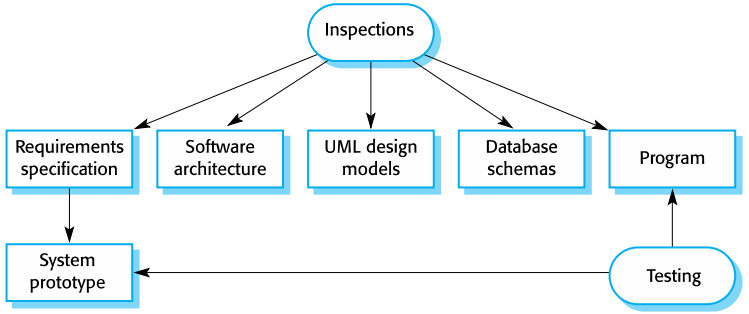
\includegraphics[width=0.65\linewidth]{images/inspection-and-testing.PNG}
    \caption{Ispezioni e test}
    \label{fig:inspection-and-testing}
\end{figure}

Le ispezioni si concentrano principalmente sul codice sorgente di un sistema, ma qualsiasi rappresentazione leggibile del software, come i requisiti o un modello di progettazione, può essere ispezionata. Durante un’ispezione, si usa la conoscenza del sistema, del dominio di applicazione e del linguaggio di programmazione o modellazione per scoprire errori.

L’ispezione del software ha tre vantaggi rispetto al testing:
\begin{enumerate}
    \item Durante il testing, un errore può mascherare altri errori. Poiché l’ispezione non implica l’esecuzione del sistema, non si devono affrontare le interazioni tra errori e una singola sessione di ispezione può scoprire molti errori.
    \item Versioni incomplete di un sistema possono essere ispezionate senza costi aggiuntivi. Se un programma è incompleto, per testarlo servono “test harness” specializzati, aumentando i costi di sviluppo.
    \item Oltre a cercare difetti, un’ispezione può considerare attributi qualitativi come la conformità agli standard, la portabilità e la manutenibilità.
\end{enumerate}
Tuttavia, le ispezioni non possono sostituire il testing, poiché non sono efficaci nel rilevare difetti derivanti da interazioni impreviste tra parti diverse del programma, problemi di temporizzazione o problemi di prestazioni del sistema. Ispezioni e test sono tecniche di verifica complementari e non opposte. Entrambe dovrebbero essere utilizzate durante il processo V\&V.

In questo capitolo ci concentriamo sul testing e sui processi di testing. La Figura \ref{fig:model-software-testing-process} è un modello astratto del processo di testing tradizionale, utilizzato nello sviluppo guidato dalla pianificazione. I casi di test sono specifiche degli input e degli output attesi dal sistema (i risultati del test), insieme a una dichiarazione di ciò che viene testato. I dati di test sono gli input ideati per testare un sistema. L’esecuzione del test può essere automatizzata, e i risultati del test vengono confrontati automaticamente con quelli previsti.

\begin{figure}[ht]
    \centering
    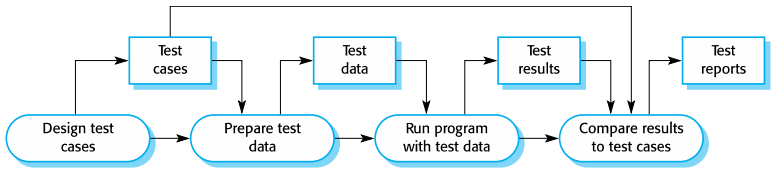
\includegraphics[width=0.75\linewidth]{images/model-software-testing-process.PNG}
    \caption{Un modello del processo di test del software}
    \label{fig:model-software-testing-process}
\end{figure}

In genere, un sistema software commerciale passa attraverso tre fasi di testing:
\begin{enumerate}
    \item Testing durante lo sviluppo, dove il sistema viene testato durante lo sviluppo per scoprire bug e difetti.
    \item Testing della versione, dove un team di test separato testa una versione completa del sistema prima che venga rilasciata agli utenti.
    \item Testing dell'utente, in cui gli utenti o potenziali utenti testano il sistema nel loro ambiente.
\end{enumerate}

\section{Test di sviluppo}
Il testing durante lo sviluppo include tutte le attività di testing che vengono svolte dal team che sviluppa il sistema.

Ci sono tre fasi di testing durante lo sviluppo:
\begin{enumerate}
    \item \textit{Testing dell’unità}, in cui vengono testate singole unità del programma o classi di oggetti. Il testing dell’unità dovrebbe concentrarsi sul test delle funzionalità degli oggetti o dei metodi.
    \item \textit{Testing del componente}, in cui vengono integrate diverse unità per creare componenti compositi. Il testing del componente dovrebbe concentrarsi sul test delle interfacce del componente, che forniscono accesso alle funzioni del componente.
    \item \textit{Testing del sistema}, in cui alcuni o tutti i componenti di un sistema vengono integrati e il sistema viene testato nel suo complesso. Il testing del sistema dovrebbe concentrarsi sul test delle interazioni tra i componenti.
\end{enumerate}

\subsection{Unit testing}
Il testing dell’unità è il processo di test dei componenti del programma, come metodi o classi di oggetti. Le singole funzioni o metodi sono il tipo più semplice di componente. I test dovrebbero consistere in chiamate a queste routine con diversi parametri di input.

Quando si testano classi di oggetti, è necessario progettare i test in modo da coprire tutte le funzionalità dell'oggetto. Ciò significa che bisogna testare tutte le operazioni associate all'oggetto, impostare e controllare il valore di tutti gli attributi associati e mettere l'oggetto in tutti gli stati possibili. In questo modo, si simuleranno tutti gli eventi che causano un cambiamento di stato.

Ad esempio, l'oggetto stazione meteorologica. Gli attributi e le operazioni di questo oggetto sono mostrati nella Figura \ref{fig:weather-station-object}. Ha un solo attributo, che è il suo identificatore. È quindi necessario solo un test per verificare che sia stata configurata correttamente. Bisogna definire casi di test per tutti i metodi associati all'oggetto, come \texttt{reportWeather} e \texttt{reportStatus}. Idealmente, i metodi dovrebbero essere testati isolatamente, ma in alcuni casi sono necessarie sequenze di test. Ad esempio, per testare il metodo che spegne gli strumenti della stazione meteorologica (\texttt{shutdown}), è necessario prima aver eseguito il metodo \texttt{restart}.

\begin{figure}[ht]
    \centering
    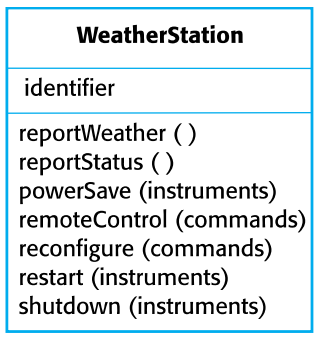
\includegraphics[width=0.25\linewidth]{images/weather-station-object.PNG}
    \caption{Test della stazione meteorologica}
    \label{fig:weather-station-object}
\end{figure}

Per testare gli stati della stazione meteorologica, si può utilizzare un modello di stato. Utilizzando questo modello, si identificano sequenze di transizioni di stato che devono essere testate e si definiscono sequenze di eventi per forzare queste transizioni. Esempi di sequenze di stato da testare nella stazione meteorologica includono:
\begin{itemize}
    \item \texttt{Shutdown} $\to$ \texttt{Running} $\to$ \texttt{Shutdown}
    \item \texttt{Configuring} $\to$ \texttt{Running} $\to$ \texttt{Testing} $\to$ \texttt{Transmitting} $\to$ \texttt{Running}
    \item \texttt{Running} $\to$ \texttt{Collecting} $\to$ \texttt{Running} $\to$ \texttt{Summarizing} $\to$ \texttt{Transmitting} $\to$ \texttt{Running}
\end{itemize}
Quando possibile, il testing dell’unità dovrebbe essere automatizzato. Nel testing dell’unità automatizzato, si utilizza un framework di automazione del test, come JUnit per scrivere ed eseguire i test del programma. I framework di testing dell’unità forniscono classi di test generiche che possono essere estese per creare casi di test specifici. Possono quindi eseguire tutti i test implementati e riportare, spesso tramite un’interfaccia grafica (GUI), il successo o meno dei test.

Un test automatizzato ha tre parti:
\begin{enumerate}
    \item Una \textit{parte di configurazione}, dove si inizializza il sistema con il caso di test, ovvero gli input e gli output attesi.
    \item Una \textit{parte di chiamata}, dove si chiama l'oggetto o il metodo da testare.
    \item Una \textit{parte di asserzione}, dove si confronta il risultato della chiamata con il risultato atteso. Se l’asserzione è vera, il test ha avuto successo; se è falsa, il test è fallito.
\end{enumerate}

\subsection{Scelta dei casi di unit test}
Il testing è costoso e richiede tempo, quindi è importante scegliere casi di test dell’unità efficaci. L'efficacia, in questo caso, implica due aspetti:
\begin{enumerate}
    \item I casi di test dovrebbero dimostrare che, quando usato come previsto, il componente testato fa ciò che dovrebbe fare.
    \item Se ci sono difetti nel componente, questi dovrebbero essere rivelati dai casi di test.
\end{enumerate}
È quindi necessario progettare due tipi di casi di test. Il primo dovrebbe riflettere il funzionamento normale del programma e dimostrare che il componente funziona. L’altro tipo di caso di test dovrebbe basarsi sull’esperienza, prendendo in considerazione i problemi più comuni. Dovrebbe utilizzare input anomali per verificare che siano correttamente processati e non mandino in crash il componente.

Due strategie efficaci per scegliere i casi di test sono:
\begin{enumerate}
    \item \textit{Testing per partizione}, in cui si identificano gruppi di input con caratteristiche comuni e che devono essere processati allo stesso modo. I test vengono scelti all'interno di ciascun gruppo.
    \item \textit{Testing basato su linee guida}, in cui si utilizzano linee guida per scegliere i casi di test. Queste linee guida riflettono l’esperienza precedente riguardo ai tipi di errori che i programmatori spesso commettono nello sviluppo dei componenti.
\end{enumerate}
Gli input e gli output di un programma possono essere considerati come membri di insiemi con caratteristiche comuni. I programmi di solito si comportano in modo simile per tutti i membri di un insieme.

A causa di questo comportamento equivalente, queste classi vengono talvolta chiamate partizioni di equivalenza o domini. Un approccio sistematico alla progettazione dei casi di test si basa sull’identificazione di tutte le partizioni di input e output per un sistema o componente. I casi di test sono progettati in modo che gli input o gli output rientrino in queste partizioni. 

Nella Figura \ref{fig:equivalence-partitioning}, l'ellisse grande a sinistra rappresenta l’insieme di tutti gli input possibili per il programma che viene testato. Le ellissi più piccole rappresentano le partizioni di equivalenza. Un programma in fase di test dovrebbe processare tutti i membri di una partizione di equivalenza di input allo stesso modo. Le partizioni di equivalenza di output sono partizioni in cui tutti gli output hanno qualcosa in comune.

\begin{figure}[ht]
    \centering
    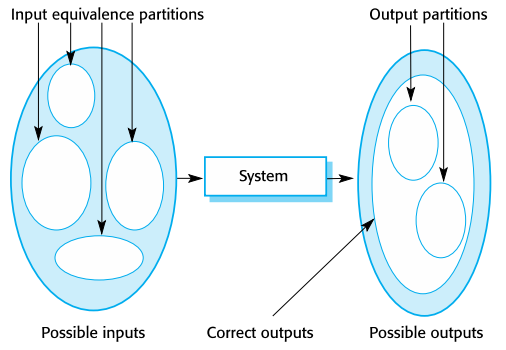
\includegraphics[width=0.50\linewidth]{images/equivalence-partitioning.PNG}
    \caption{Partizionamento di equivalenza}
    \label{fig:equivalence-partitioning}
\end{figure}

Una volta identificato un insieme di partizioni, si scelgono casi di test da ciascuna di queste partizioni. Una buona regola per la selezione dei casi di test è scegliere casi ai confini delle partizioni, più alcuni vicini al punto medio della partizione. 

Si identificano le partizioni utilizzando la specifica del programma o la documentazione utente e, in base all’esperienza, prevedendo le classi di valori di input che potrebbero rilevare errori. Ad esempio, si supponga che una specifica di programma stabilisca che il programma accetta da quattro a otto input costituiti da numeri interi di cinque cifre maggiori di 10.000. Si utilizza questa informazione per identificare le partizioni di input e i possibili valori di test. Questi sono mostrati nella Figura \ref{fig:equivalence-partitioning2}.

\begin{figure}[ht]
    \centering
    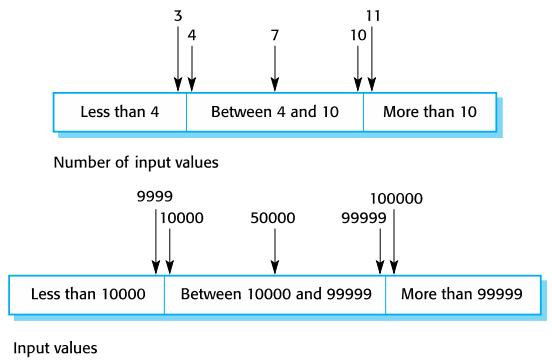
\includegraphics[width=0.55\linewidth]{images/equivalence-partitioning2.PNG}
    \caption{Esempio di partizionamento di equivalenza}
    \label{fig:equivalence-partitioning2}
\end{figure}

È anche possibile utilizzare le linee guida di testing per scegliere i casi di test. Le linee guida raccolgono conoscenze sui tipi di casi di test efficaci per la rilevazione di errori. Ad esempio, quando si testano programmi con sequenze, array o liste, alcune linee guida che potrebbero rivelare difetti includono:
\begin{enumerate}
    \item Testare il software con sequenze che contengono solo un singolo valore.
    \item Utilizzare sequenze di dimensioni diverse in test diversi.
    \item Derivare test in modo che il primo, il mezzo e l’ultimo elemento della sequenza siano accessibili.
\end{enumerate}
Alcune delle linee guida più generali che suggerisce sono:
\begin{enumerate}
    \item Scegliere input che costringano il sistema a generare tutti i messaggi di errore.
    \item Progettare input che causino l’overflow dei buffer di input.
    \item Ripetere più volte lo stesso input o una serie di input.
    \item Forzare la generazione di output non validi.
    \item Forzare i risultati del calcolo a essere troppo grandi o troppo piccoli.
\end{enumerate}

\subsection{Testing dei componenti}
I componenti software sono spesso costituiti da diversi oggetti che interagiscono tra loro. Ad esempio, nel sistema della stazione meteorologica, il componente di riconfigurazione include oggetti che gestiscono ciascun aspetto della riconfigurazione. L’accesso alla funzionalità di questi oggetti avviene tramite le interfacce dei componenti. Il testing dei componenti compositi dovrebbe quindi concentrarsi sul dimostrare che l'interfaccia o le interfacce del componente si comportano secondo la specifica. Si può supporre che i test delle singole unità sugli oggetti all'interno del componente siano stati completati.

La Figura \ref{fig:interface-testing} illustra l'idea di test dell'interfaccia del componente. Supponiamo che i componenti A, B e C siano stati integrati per creare un componente o sottosistema più grande. I casi di test non vengono applicati ai singoli componenti, ma all’interfaccia del componente composito creato combinando questi componenti.

\begin{figure}[ht]
    \centering
    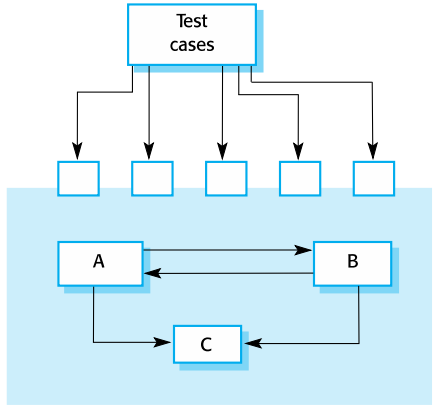
\includegraphics[width=0.40\linewidth]{images/interface-testing.PNG}
    \caption{Test dell'interfaccia}
    \label{fig:interface-testing}
\end{figure}

Esistono diversi tipi di interfaccia tra i componenti del programma e, di conseguenza, diversi tipi di errore d’interfaccia che possono verificarsi:
\begin{enumerate}
    \item \textit{Interfacce a parametri:} sono interfacce in cui vengono passati dati o, talvolta, riferimenti a funzioni da un componente all'altro.
    \item \textit{Interfacce a memoria condivisa:} sono interfacce in cui un blocco di memoria è condiviso tra i componenti.
    \item \textit{Interfacce procedurali:} sono interfacce in cui un componente incapsula un insieme di procedure che possono essere chiamate da altri componenti.
    \item \textit{Interfacce di passaggio di messaggi:} sono interfacce in cui un componente richiede un servizio da un altro componente inviandogli un messaggio.
\end{enumerate}
Gli errori d’interfaccia sono una delle forme più comuni di errore nei sistemi complessi. Questi errori si dividono in tre categorie:
\begin{enumerate}
    \item \textit{Uso improprio dell’interfaccia:} un componente chiamante richiama un altro componente e commette un errore nell'uso della sua interfaccia. Questo tipo di errore è comune nelle interfacce a parametri, dove i parametri possono essere del tipo sbagliato o passati nell'ordine sbagliato, oppure il numero di parametri passati può essere errato.
    \item \textit{Incomprensione dell’interfaccia:} un componente chiamante fraintende la specifica dell’interfaccia del componente chiamato e fa ipotesi sul suo comportamento.
    \item \textit{Errori di sincronizzazione:}il produttore di dati e il consumatore di dati possono operare a velocità diverse o può accedere a informazioni non aggiornate.
\end{enumerate}
Alcune linee guida generali per il testing delle interfacce sono:
\begin{enumerate}
    \item Progettare una serie di test in cui i valori dei parametri per i componenti esterni si trovino agli estremi dei loro intervalli.
    \item Quando vengono passati puntatori tramite un’interfaccia, testare sempre l’interfaccia con parametri puntatori nulli.
    \item Progettare test che causino deliberatamente il fallimento del componente.
    \item Usare il testing di stress nei sistemi di passaggio di messaggi.
    \item Quando più componenti interagiscono tramite memoria condivisa, progettare test che variano l'ordine in cui questi componenti vengono attivati.
\end{enumerate}

\subsection{Testing del sistema}
Il testing del sistema durante lo sviluppo prevede l'integrazione dei componenti per creare una versione del sistema e poi testare il sistema integrato. Il testing del sistema verifica che i componenti siano compatibili, interagiscano correttamente e trasferiscano i dati giusti al momento giusto attraverso le loro interfacce. Ovviamente si sovrappone al testing dei componenti, ma ci sono due differenze importanti:
\begin{enumerate}
    \item Durante il testing del sistema, i componenti riutilizzabili che sono stati sviluppati separatamente e i sistemi commerciali possono essere integrati con componenti di nuova progettazione. Successivamente viene testato il sistema completo.
    \item In questa fase possono essere integrati componenti sviluppati da diversi membri del team o sottoteam. Il testing del sistema è un processo collettivo piuttosto che individuale. In alcune aziende, il testing del sistema può coinvolgere un team di testing separato senza il coinvolgimento di designer e programmatori.
\end{enumerate}
Grazie alla sua attenzione alle interazioni, il testing basato sui casi d'uso è un approccio efficace per il testing del sistema. Di solito diversi componenti o oggetti implementano ciascun caso d'uso nel sistema. Il testing del caso d'uso forza queste interazioni. Se si è sviluppato un diagramma di sequenza per modellare l’implementazione del caso d'uso, si possono vedere gli oggetti o i componenti coinvolti nell'interazione.

Nel caso di esempio della stazione meteorologica, il software di sistema riporta dati meteorologici riassunti a un computer remoto. La Figura \ref{fig:collect-weather-data-sequence-chart} mostra la sequenza di operazioni nella stazione meteorologica quando risponde a una richiesta di raccolta dati per il sistema di mappatura. 

\begin{figure}[ht]
    \centering
    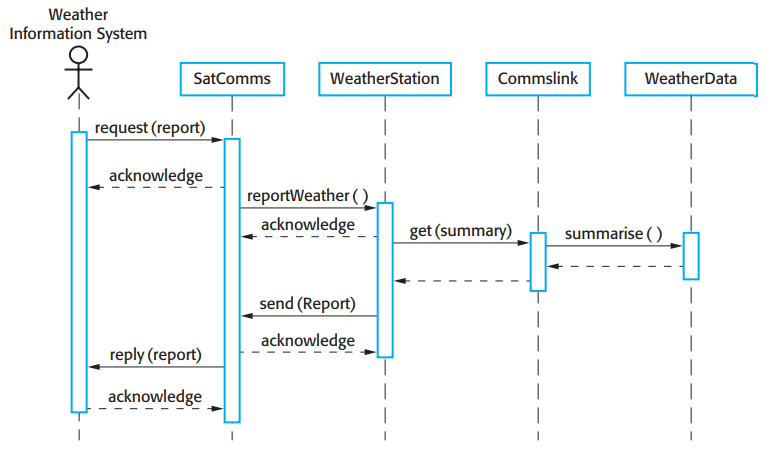
\includegraphics[width=0.70\linewidth]{images/collect-weather-data-sequence-chart.PNG}
    \caption{Raccogliere la sequenza dei dati meteorologici}
    \label{fig:collect-weather-data-sequence-chart}
\end{figure}

Pertanto, emettere una richiesta per un report comporterà l'esecuzione della seguente sequenza di metodi: 
\begin{align*}
\texttt{SatComms:request} \to \texttt{WeatherStation:reportWeather} \to \texttt{Commslink:Get(summary)} \to\\\texttt{WeatherData:summarize}
\end{align*}
Il diagramma di sequenza aiuta a progettare i casi di test specifici di cui si ha bisogno, poiché mostra quali input sono richiesti e quali output vengono creati:
\begin{enumerate}
    \item Un input di una richiesta per un report dovrebbe avere un riconoscimento associato. Da una richiesta dovrebbe essere infine restituito un report. Durante il testing, si dovrebbero creare dati riassunti che possono essere utilizzati per verificare che il report sia organizzato correttamente.
    \item Una richiesta di input per un report a \texttt{WeatherStation} risulta nella generazione di un report riassunto. Si può testare questo in isolamento creando dati grezzi corrispondenti al riepilogo preparato per il test di \texttt{SatComms} e verificando che l'oggetto \texttt{WeatherStation} produca correttamente questo riepilogo. Questi dati grezzi vengono utilizzati anche per testare l'oggetto \texttt{WeatherData}.
\end{enumerate}
Il testing esaustivo, in cui viene testata ogni possibile sequenza di esecuzione del programma, è impossibile. Il testing, quindi, deve basarsi su un sottoinsieme dei possibili casi di test. Ad esempio:
\begin{enumerate}
    \item Tutte le funzioni del sistema accessibili tramite menu dovrebbero essere testate.
    \item Le combinazioni di funzioni (ad esempio, la formattazione del testo) che sono accessibili dallo stesso menu devono essere testate.
    \item Dove è previsto l’input dell’utente, tutte le funzioni devono essere testate sia con input corretto che con input errato.
\end{enumerate}

\section{Test-driven developement}
Lo sviluppo guidato dai test (Test-Driven Developement - TDD) è un approccio allo sviluppo del software in cui si alternano la scrittura dei test e lo sviluppo del codice. Si sviluppa il codice in modo incrementale, insieme a un set di test per ogni incremento. Non si inizia a lavorare sul prossimo incremento finché il codice sviluppato non supera tutti i test. Lo sviluppo guidato dai test è stato introdotto come parte del metodo di sviluppo agile. Tuttavia, oggi è ampiamente accettato e può essere utilizzato sia in processi agili che pianificati.

Il processo fondamentale di TDD è mostrato nella Figura \ref{fig:test-driven-development}. I passaggi del processo sono i seguenti:

\begin{figure}[ht]
    \centering
    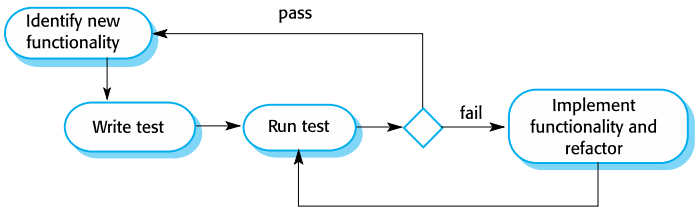
\includegraphics[width=0.57\linewidth]{images/test-driven-development.PNG}
    \caption{Sviluppo basato sui test}
    \label{fig:test-driven-development}
\end{figure}

\begin{enumerate}
    \item Si inizia identificando l'incremento di funzionalità richiesto. Questo dovrebbe essere normalmente piccolo e implementabile in poche righe di codice.
    \item Si scrive un test per questa funzionalità e lo si implementa come un test automatizzato.
    \item Successivamente, si esegue il test, insieme a tutti gli altri test che sono stati implementati. Inizialmente, non si è implementata la funzionalità, quindi il nuovo test fallirà.
    \item Si implementa quindi la funzionalità e si riesegue il test.
    \item Una volta che tutti i test passano con successo, si passa all'implementazione del prossimo blocco di funzionalità.
\end{enumerate}
Oltre a una migliore comprensione del problema, altri vantaggi dello sviluppo guidato dai test sono:
\begin{enumerate}
    \item \textit{Copertura del codice.} In linea di principio, ogni segmento di codice che si scrive dovrebbe avere almeno un test associato.
    \item \textit{Testing di regressione.} Un set di test viene sviluppato in modo incrementale man mano che il programma viene sviluppato.
    \item \textit{Debugging semplificato.} Quando un test fallisce, dovrebbe essere ovvio dove si trova il problema. Il codice appena scritto deve essere controllato e modificato.
    \item \textit{Documentazione del sistema.} I test stessi fungono da una forma di documentazione che descrive cosa dovrebbe fare il codice.
\end{enumerate}
Uno dei vantaggi più importanti del TDD è che riduce i costi del testing di regressione. Il testing di regressione comporta l'esecuzione di set di test che sono stati eseguiti con successo dopo che sono state apportate modifiche a un sistema. Il test di regressione verifica che queste modifiche non abbiano introdotto nuovi bug nel sistema e che il nuovo codice interagisca come previsto con il codice esistente. Il testing di regressione è costoso e a volte impraticabile quando un sistema viene testato manualmente, poiché i costi in termini di tempo e sforzo sono molto alti. Il testing automatizzato riduce drasticamente i costi del testing di regressione. Dopo aver apportato una modifica a un sistema nello sviluppo test-first, tutti i test esistenti devono passare con successo prima che venga aggiunta altra funzionalità.

\section{Testing di rilascio}
Il testing di rilascio è il processo di test di una particolare versione di un sistema destinata all'uso al di fuori del team di sviluppo. Normalmente, la release del sistema è destinata a clienti e utenti. Tuttavia, in un progetto complesso, la release potrebbe essere destinata ad altri team che stanno sviluppando sistemi correlati.

Ci sono due importanti differenze tra il testing di rilascio e il testing di sistema durante il processo di sviluppo:
\begin{enumerate}
    \item Il team di sviluppo del sistema non dovrebbe essere responsabile del testing di rilascio.
    \item Il testing di rilascio è un processo di verifica per assicurarsi che un sistema soddisfi i suoi requisiti e sia sufficientemente buono per l'uso da parte dei clienti del sistema.
    
    Il testing di sistema eseguito dal team di sviluppo dovrebbe concentrarsi sul trovare bug nel sistema (defect testing).
\end{enumerate}
L'obiettivo principale del processo di testing di rilascio è convincere il fornitore del sistema che esso sia sufficientemente buono per l'uso. Se è così, può essere rilasciato come prodotto o consegnato al cliente. Il testing di rilascio, quindi, deve dimostrare che il sistema fornisce la funzionalità, le prestazioni e l'affidabilità specificate e che non fallisce durante l'uso normale.

Il testing di rilascio è di solito un processo di testing black-box in cui i test vengono derivati dalle specifiche del sistema. Il sistema viene trattato come una "scatola nera" il cui comportamento può essere determinato solo studiando i suoi input e gli output correlati.

\subsection{Testing basato sui requisiti}
Un principio generale di buona pratica nell'ingegneria dei requisiti è che i requisiti dovrebbero essere testabili. Questo significa che il requisito dovrebbe essere scritto in modo tale che sia possibile progettare un test per quel requisito.

Ad esempio, consideriamo i seguenti requisiti del sistema Mentcare riguardanti il controllo delle allergie ai farmaci:
\begin{itemize}
    \item Se un paziente è noto per essere allergico a un particolare farmaco, la prescrizione di quel farmaco deve generare un messaggio di avviso per l'utente del sistema.
    \item Se chi prescrive sceglie di ignorare un avviso di allergia, deve fornire una motivazione per questa scelta.
\end{itemize}
Per verificare se questi requisiti sono stati soddisfatti, potrebbero essere necessari diversi test correlati:
\begin{enumerate}
    \item Creare un record del paziente senza allergie note. Prescrivere farmaci per allergie note e verificare che il sistema non generi un messaggio di avviso.
    \item Creare un record del paziente con un'allergia nota. Prescrivere il farmaco a cui il paziente è allergico e verificare che il sistema generi un avviso.
    \item Creare un record del paziente in cui siano registrate allergie a due o più farmaci. Prescrivere separatamente entrambi i farmaci e verificare che il sistema generi correttamente l'avviso per ciascun farmaco.
    \item Prescrivere due farmaci a cui il paziente è allergico. Verificare che il sistema emetta correttamente due avvisi.
    \item Prescrivere un farmaco che genera un avviso e ignorare quell'avviso. Verificare che il sistema richieda all'utente di fornire una spiegazione del motivo per cui l'avviso è stato ignorato.
\end{enumerate}

\subsection{Testing basato su scenari}
Il testing basato su scenari è un approccio al testing di rilascio in cui si creano scenari tipici di utilizzo e si usano questi scenari per sviluppare casi di test per il sistema. Uno scenario è una storia realistica e facilmente compresibile che descrive un modo in cui il sistema potrebbe essere utilizzato.

\begin{Example}{Scenario per il sistema Mentcare}{}
\textit{George è un infermiere specializzato in assistenza sanitaria mentale. Una delle sue responsabilità è visitare i pazienti a domicilio per verificare che il loro trattamento sia efficace e che non soffrano di effetti collaterali dovuti ai farmaci.}

\textit{In una giornata dedicata alle visite domiciliari, George accede al sistema Mentcare e lo utilizza per stampare il programma delle visite domiciliari previste per quella giornata, insieme a informazioni riepilogative sui pazienti da visitare. Richiede che i record di questi pazienti vengano scaricati sul suo laptop e gli viene richiesto di inserire la sua frase chiave per criptare i record sul laptop.}

\textit{Uno dei pazienti che visita è Jim, che viene trattato con farmaci per la depressione. Jim ritiene che la terapia lo stia aiutando, ma crede che gli causi insonnia. George consulta il record di Jim e viene invitato a inserire la sua frase chiave per decrittare il record. Controlla il farmaco prescritto e verifica i suoi effetti collaterali. L'insonnia è un effetto collaterale noto, quindi annota il problema nel record di Jim e gli suggerisce di recarsi in clinica per cambiare farmaco. Jim è d'accordo, così George inserisce un promemoria per contattarlo al suo ritorno in clinica e fissare un appuntamento con un medico. George conclude la consultazione e il sistema recripta il record di Jim.}

\textit{Dopo aver terminato le consultazioni, George torna in clinica e carica i record dei pazienti visitati nel database. Il sistema genera una lista di chiamate per George, che include i pazienti da contattare per raccogliere informazioni di follow-up e per fissare appuntamenti in clinica.}
\end{Example}

Questo scenario testa diverse funzionalità del sistema Mentcare:
\begin{enumerate}
    \item Autenticazione tramite accesso al sistema.
    \item Scaricamento e caricamento dei record dei pazienti su un laptop.
    \item Pianificazione delle visite a domicilio.
    \item Crittografia e decrittografia dei record dei pazienti su un dispositivo mobile.
    \item Recupero e modifica dei record.
    \item Collegamenti con il database dei farmaci che mantiene le informazioni sugli effetti collaterali.
    \item Sistema di promemoria per le chiamate.
\end{enumerate}

\subsection{Testing delle prestazioni}
Una volta che un sistema è stato completamente integrato, è possibile testare proprietà emergenti, come prestazioni e affidabilità. I test delle prestazioni devono essere progettati per garantire che il sistema possa gestire il carico previsto. Ciò di solito comporta una serie di test in cui si aumenta il carico fino a quando le prestazioni del sistema diventano inaccettabili.

Lo stress testing permette di testare il comportamento del sistema in caso di guasto e 
rivelare difetti che si manifestano solo quando il sistema è completamente carico.

\section{Testing dell'utente}
Il test dell'utente o del cliente è una fase del processo di testing in cui gli utenti o i clienti forniscono feedback e consigli sui test del sistema. Il test dell'utente è essenziale, anche quando sono stati effettuati test di sistema e di rilascio completi, poiché l'ambiente di lavoro dell'utente può influire notevolmente su affidabilità, prestazioni, usabilità e robustezza del sistema.

È praticamente impossibile per uno sviluppatore replicare l'ambiente di lavoro del sistema. Ad esempio, un sistema destinato all'uso in un ospedale opera in un ambiente clinico dove avvengono altre attività, come emergenze dei pazienti e conversazioni con i familiari. Questi fattori influenzano l'uso del sistema, ma gli sviluppatori non possono includerli nel loro ambiente di test.

Esistono tre diversi tipi di test dell'utente:
\begin{enumerate}
    \item \textit{Test alpha}, in cui un gruppo selezionato di utenti collabora strettamente con il team di sviluppo per testare le prime versioni del software.
    \item \textit{Test beta}, in cui una versione del software viene resa disponibile a un gruppo più ampio di utenti per permettere loro di sperimentare e segnalare eventuali problemi ai sviluppatori del sistema.
    \item \textit{Test di accettazione}, in cui i clienti testano un sistema per decidere se accettarlo o meno dai sviluppatori e implementarlo nel loro ambiente.
\end{enumerate}
    \label{fig:acceptance-testing-process}
Le fasi nel processo di test di accettazione sono sei (Figura \ref{fig:acceptance-testing-process}):

\begin{figure}[ht]
    \centering
    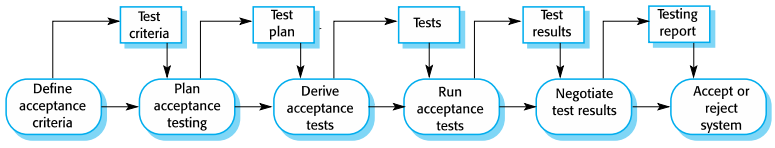
\includegraphics[width=0.75\linewidth]{images/acceptance-testing-process.PNG}
    \caption{Il processo di test di accettazione}
    \label{fig:acceptance-testing-process}
\end{figure}

\begin{enumerate}
    \item \textit{Definizione dei criteri di accettazione:} questa fase dovrebbe idealmente svolgersi all'inizio, prima della firma del contratto per il sistema.
    \item \textit{Pianificazione del test di accettazione:} include risorse, tempo e budget, e stabilisce un programma di test.
    \item \textit{Progettazione dei test di accettazione:} i test sono progettati per verificare che il sistema sia accettabile, sia per le caratteristiche funzionali che non funzionali.
    \item \textit{Esecuzione dei test di accettazione:} i test vengono eseguiti sul sistema, idealmente nell'ambiente reale in cui verrà utilizzato.
    \item \textit{Negoziazione dei risultati dei test:} poiché difficilmente tutti i test di accettazione saranno superati senza problemi, cliente e sviluppatore devono negoziare per decidere se il sistema è accettabile.
    \item \textit{Rifiuto/accettazione del sistema:} incontro tra sviluppatori e cliente per decidere se accettare il sistema o richiedere ulteriori sviluppi.
\end{enumerate}
Nei metodi agili  potrebbe non esserci una fase separata per il test di accettazione. L'utente finale è parte del team di sviluppo e fornisce i requisiti del sistema in termini di user stories, definendo anche i test per verificare se il software sviluppato le supporta. Questi test sono equivalenti ai test di accettazione e vengono automatizzati; lo sviluppo non procede fino a quando i test di accettazione delle user stories non sono stati superati.

Tuttavia, trovare utenti "tipici" può essere difficile, e i test di accettazione possono non riflettere appieno come un sistema venga effettivamente utilizzato.

\section{Punti chiave}
\begin{center}
\begin{minipage}{\textwidth}
\colorbox{lightgray}{
\parbox{\linewidth}{
\begin{itemize} 
    \item Il testing può solo mostrare la presenza di errori in un programma. Non può dimostrare che non ci siano più difetti.
    \item Il testing durante lo sviluppo è responsabilità del team di sviluppo software. Un team separato dovrebbe essere incaricato di testare un sistema prima che venga rilasciato ai clienti.
    \item Il testing durante lo sviluppo include: il testing unitario, in cui vengono testati singoli oggetti e metodi; il testing dei componenti, in cui vengono testati gruppi correlati di oggetti; il testing del sistema, in cui vengono testati sistemi parziali o completi.
    \item Quando si testa il software, bisogna cercare di "romperlo" usando l’esperienza e le linee guida per scegliere tipi di casi di test che si sono dimostrati efficaci nello scoprire difetti in altri sistemi.
    \item Quando possibile, è preferibile scrivere test automatizzati. I test vengono integrati in un programma che può essere eseguito ogni volta che viene apportata una modifica a un sistema.
    \item Sviluppo orientato ai test è un approccio di sviluppo in cui i test vengono scritti prima del codice da testare.
    \item Il testing basato su scenari prevede l’invenzione di uno scenario di utilizzo tipico e l’uso di questo scenario per derivare i casi di test.
    \item Il testing di accettazione è un processo di testing condotto dall'utente, con l’obiettivo di stabilire se il software è sufficientemente buono per essere implementato e utilizzato nel suo ambiente operativo.
\end{itemize}
}}
\end{minipage}
\end{center}